\documentclass{deliverablereport}
\usepackage[show]{ed}
\usepackage{paralist}
\def\dmh{\texttt{data.mathub.info}\xspace}

\usepackage[style=alphabetic,backend=bibtex]{biblatex}
\addbibresource{../../lib/kbibs/kwarcpubs.bib}
\addbibresource{../../lib/kbibs/extpubs.bib}
\addbibresource{../../lib/kbibs/kwarccrossrefs.bib}
\addbibresource{../../lib/kbibs/extcrossrefs.bib}
\addbibresource{../../lib/deliverables.bib}
\addbibresource{local.bib}
\renewbibmacro*{event+venue+date}{}
\renewbibmacro*{doi+eprint+url}{%
  \iftoggle{bbx:doi}
    {\printfield{doi}\iffieldundef{doi}{}{\clearfield{url}}}
    {}%
  \newunit\newblock
  \iftoggle{bbx:eprint}
    {\usebibmacro{eprint}}
    {}%
  \newunit\newblock
  \iftoggle{bbx:url}
    {\usebibmacro{url+urldate}}
    {}}

\deliverable{management}{imp2}
\duedate{31/05/2019 (M45)}
\deliverydate{06/09/2019}

\author{Nicolas M. Thiéry et al.}

\begin{document}
\enlargethispage{4ex}
\maketitle
\githubissuedescription
\clearpage
\tableofcontents
\clearpage


\section{Context}

OpenDreamKit (Open Digital Research Environment Toolkit, \ODK for
short) is a four-year Horizon 2020 European Research Infrastructure
project (\#676541). In the 2015-2019 period, it provided substantial funding to the open-source
computational mathematics ecosystem, and in particular popular tools
such as \Linbox, \MPIR, \Sage, \GAP, \PariGP, \LMFDB, \Singular,
\MathHub, and the \Jupyter interactive computing environment.

From this ecosystem, \ODK has delivered a flexible toolkit
enabling research groups to set up Virtual Research Environments
(VRE), customised to meet the varied needs of research projects in
pure mathematics and applications, and supporting the full research
life-cycle from exploration, through proof and publication, to
archival and sharing of data and code.

The primary end-users are researchers in (pure) mathematics; however,
thanks to the modular design the work will benefit a wide range of
end-users, including teachers, engineers, in academia, public
institutions, or enterprises.

An unusual feature of \ODK is that it emerged from an ecosystem of
community-developed software where the prevalent development model is
``by users for users''. And indeed, many of the \ODK participants are
themselves end-users: academics wearing several hats -- developer,
researcher, teacher, in mathematics or computer science, etc. -- who
gathered to develop the computational tools they needed for their daily
research. \ODK itself was born from two dual movements,
developers pushing innovation and end-users pulling innovation,
often led again by people wearing both hats. This, combined with long
dissemination experience from said people, is a strong asset for
delivering products which actually benefit a wide range of end-users.

Reciprocally, \ODK works hand-in-hand with relevant communities; some
innovations brought to the toolkit are partially or entirely
accomplished outside of the \ODK project. This is not a
problem in itself as the communities and the project share the same
values and objectives.

End-users will benefit from innovations brought by \ODK in the
multiple pieces of software forming the open-source VRE. In the case of
ODK the innovation will be the unification of open-source
tools with overlapping functionality, the simplification of the tools
for end-users without coding expertise, and the development of
user-friendly interfaces.

The following document reviews the innovations that \ODK brings to
end-users, then explains the processes enabling the implementation of
said innovations, and how \ODK targets its end-users. Most of the usual
Intellectual Property issues were easily taken care of in this project
thanks to the systematic use of open licenses; a few caveats exist
nevertheless and we briefly discuss the choice of licenses,
exemplifying potential issues with concrete examples where the project
was impacted. We conclude by reviewing the different types of outcome
of the project and discuss their respective sustainability.

\section{Innovations \ODK brings to the research community}

ODK has several cross-cutting objectives, each of which
brings innovation to the research community:
\begin{itemize}
\item{Develop and standardise math software and data for VRE: WP3, WP4, WP5, WP6}
\item{Develop core VRE components: WP3, WP4, WP5, WP6}
\item{Bring together communities: WP2, WP3}
\item{Update a range of software: WP3, WP5}
\item{Foster a sustainable ecosystem: WP3, WP4, WP5, WP6}
\item{Identify and extend ontologies: WP6}
\item{Effectiveness of the VRE: WP2}
\item{Effective dissemination: WP2}
\end{itemize}
\clearpage

We explore four typical areas of innovation in more detail:
\begin{description}
\item[Best practices and tools for correct and reproducible research]
  In the excellent talk
  \href{https://mikecroucher.github.io/MLPM_talk/}{``Is your research
    software correct''}, Mike Croucher highlights crucial best
  practices for the use of software in research, including open code
  and data sharing, automation, use of high level languages, software
  training, version control, pair programming, literate computing, and thorough
  testing. A lot of work in \ODK relates to disseminating this set of
  best practices (\longWPref{dissem}), and enabling it through
  appropriate technology (\longWPref{UI}).  Just to cite a few
  examples, \longdelivref{UI}{jupyter-collab}, and
  \longdelivref{UI}{jupyter-test} enable respectively version control
  and testing in the \Jupyter literate computing technology.
  Mike's talk has been delivered in several of \ODK's many training events (see
  especially \longdelivref{dissem}{workshops-1} and
  \longdelivref{dissem}{workshops-3}).
  \smallskip
\item[Multisystem architecture]
  Modern research increasingly requires the combination of multiple
  computational, database, and user interface components.
  We explore novel ways to combine software while taking
  advantage of parallel features, sharing data and
  semantics in a sound way, and fostering
  collaboration between systems.
  For example, a user can use the \Jupyter interface to write
  in a high-level programming language like \Sage (see \delivref{UI}{ipython-kernel-sage})
  using low-libraries like \Pari (see \taskref{UI}{pari-python})
  running high-performance computations (see \delivref{hpc}{pari-hpc2}).
  While doing this, they can access
  the Cremona database of elliptic curves, a small part of the \LMFDB
  (see \taskref{dksbases}{data-LMFDB}).
  Since all this is happening in \Jupyter, the user can easily build in
  interactivity and visualisations (see \WPref{UI}).

  \smallskip
\item[Uniform front-end to computational research results] The \Jupyter
    project -- and especially (but not limited to) the \Jupyter Notebook
    interface (formerly the IPython Notebook) -- was motivated by
    the recognition that multiple high-level, general-purpose
    programming languages in computational research (Julia, Python, R) all
    had the same need for a notebook-like format for sharing research, and that
    the existing architecture was more-or-less applicable to all three, and
    potentially many other programming languages and more specialized applications.
    We have demonstrated that, indeed, the \Jupyter notebook interface/metaphor can
    be extended to the open mathematics research community, with notebook
    interfaces for \Sage (which is already Python-based and had its own notebook
    format prior to \Jupyter), as well as more specialized CAS's with their
    own, relatively niche programming languages such as \GAP, \Pari, and \Singular.
    We have also shown the benefit of being able to reuse the same file format
    (the \texttt{ipynb} format) to share tutorials and computational research
    results across all these different systems, especially in conjunction
    with emerging technologies such as Binder, which allow execution of
    these notebooks on the cloud, with zero installation for end-users.

  \smallskip
\item[Open collaborative project preparation and management] The
  OpenDreamKit participants are long time Open Science enthusiasts.
  Accordingly, following paths that are now finally well
  established: all the project outcomes are Open Source, Open Data,
  and Open Publications. OpenDreamKit introduced one additional piece of
  innovation by exploring Open Project Management in the context of
  large European Projects: all the steps of the project ---
  preparation, production, management, reporting, dissemination ---
  were carried out in the open and in strong collaboration with the
  community.

  The outcome is overwhelmingly positive; we have actively promoted
  this approach, e.g. in the context of several blogs and
  \href{https://opendreamkit.org/2018/12/14/eu-proposal/}{presentations},
  and we hope that it will be widely adopted.
\end{description}


\section{Implementation processes of the innovations}

The organization of the innovation processes plays a key
role in the success of the software in the ecosystem \ODK builds upon.
Their
communities have, over the years if not decades, developed and
accumulated a strong expertise in the social engineering aspects of
community software development, pulling general ideas from the open-
source movement (e.g. public development, early releases, ...), and
adapting them to their specific contexts. They are heavy users of the
usual collaborative software development tools and best practices such
as mailing lists, wikis, collaborative editing pads, online chat
rooms, version control, issue trackers, continuous integration,
regression testing, code reviews, coding sprints, etc.

We describe below some striking aspects of the implementation process
in some of the software systems involved in \ODK.

\subsection{Implementation process of \Sage}

All the development happens in the open (public mailing lists, bug
tracker, ...). There is no specific sustainable leader in the
development of \Sage. Its ``community'' of developers bases its work on
the consensus of the group and on the availability of its members to
tackle issues and work on the software development. If a decision
doesn't create a consensus, there can be a vote but that seldom
happens. When any kind of change (new feature or bugfix)
is proposed to the software, it is reviewed
by at least one other member of the community, more often than not
with others looking over the shoulder.

Regarding the development process of \Sage, arguably, \ODK accelerated
trends that had just started to take a foothold before the beginning
of the project. %
Historically, all changes and additions to \Sage source code were
discussed on the issue tracker hosted at
\url{https://trac.sagemath.org}, and were only accepted after review
by a member of the community. %
While this process guaranteed the quality of the code, it also
hindered agility, a complaint often heard on \Sage forums. %
Indeed, while it is possible, with good planning and management, to
create and evolve large thematic subprojects inside \Sage (a recent
example being the Coding Theory framework), the review process still
encouraged small incremental changes over large code
removals/additions.

This workflow has nowadays evolved in two ways: first, with the
externalization of several core components to separate projects (e.g.,
UI migrated to \Jupyter, \PariGP interface migrated to CyPari, signal
handling delegated to Cysignals, \dots), the fine-grained code review
process for these now happens outside of \Sage, in the respective
issue trackers, using whatever processes and tools those projects may see
fit. %
At the level of \Sage, the quality of the included code is still
guaranteed by the standard review process at the moment of integrating
the component, however this review is much coarser, and concerned more
with integration than code quality. %
The alignment between a project's decisions and \Sage's own goals is
still guaranteed by having the \Sage community participate, or even
pilot, the development process of the component.

Second, new \Sage contributors who wanted to share their code were
historically encouraged to include it in the \Sage sources. %
While this guaranteed maximum availability of the code, it also lead
to several cases of \emph{bit-rotting} inside the \Sage codebase: old
code whose developer had left the community and that no one was
interested in keeping up to date. %
More and more, especially at \ODK dissemination events, new users are
encouraged to learn about the basics of packaging and distributing
Python code through public repositories (PyPI in particular). %
The facilities added to the \Sage executable let users easily install
packages from public repositories, thus making code sharing easy and
natural in \Sage. %
This way, end users maintain control over their \Sage projects; if one
of these projects gains enough popularity to be wanted as a basic
component of \Sage, the community can take over maintenance and
integrate it to the main code base.  This model makes it easier to
maintain a relatively stable and high-quality \emph{core} library of
basic functionality in \Sage, while giving the wider community more
agility to develop easily shareable code which \emph{uses} \Sage
without being hamstrung by the more stringent maintenance requirements
of the core library.  This is similar to the model demonstrated by the
Python \emph{standard library} itself, which places high requirements
on the inclusion of major new functionality, while preferring to
emphasize development of third-party libraries outside the standard
library. %

Experience has shown that the success of \Sage, and in particular the
biggest achievements and best innovations, owe much to a long track record of
focused week-long workshops, called \Sage Days (about ten per year
since 2005), where developers get together and form small groups for
focused coding sprints. This method is actually close to the classical
``two pizza'' team rule: "If you can't feed a team with two pizzas, it's too large";
indeed, beyond 6--7 people, the more you add people to a group,
the less the group is agile and innovative because too much effort is
put into communication and management.

\begin{figure}
  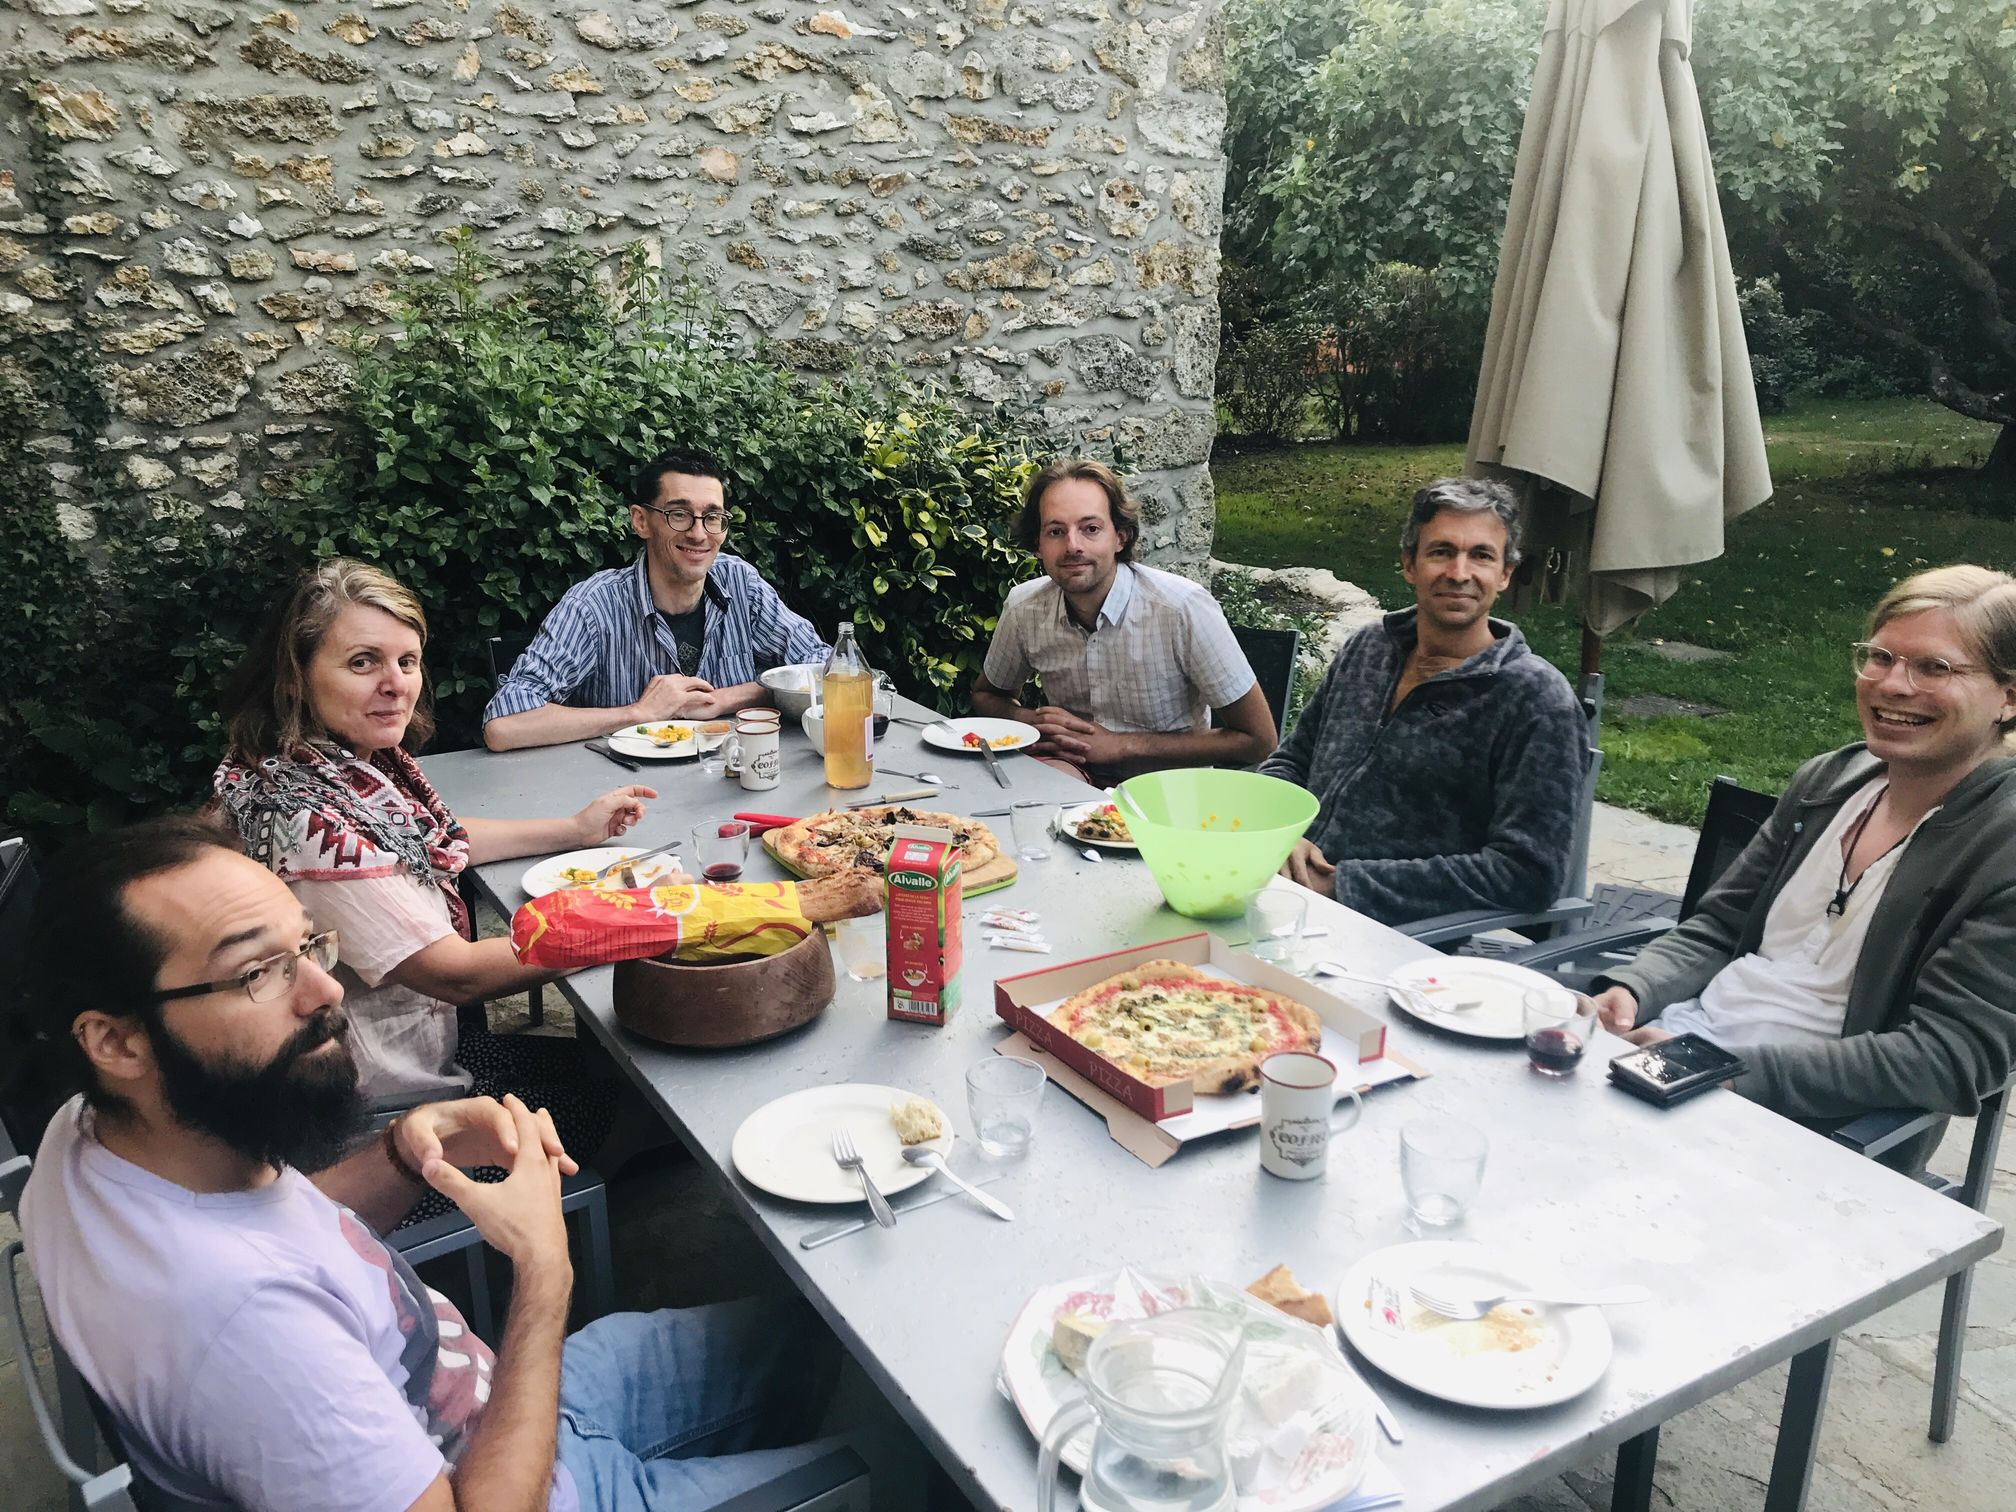
\includegraphics[width=\textwidth]{two-pizza-meal.jpg}
  \caption{A two pizza team at \ODK's end of project report writing sprint.}
\end{figure}


An example of such workshop is
\href{https://wiki.sagemath.org/days77/}{Sage Days 77}, organised by
Nicolas Thiéry in April 4--8 2016, in a guest house far from urban
civilization and with a solid internet connection. About 15 people
joined this workshop throughout the week, and split into three or four
constantly self-reorganizing teams. Concerning the impact, proper
packaging and distribution has been a recurrent issue for \Sage and is
a major task for \ODK
(\longtaskref{component-architecture}{mod-packaging}). Major
brainstorms occurred during the week to clarify the needs, isolate the
core difficulties, and explore potential approaches to tackle
them. The outcome was posted on the
\href{https://wiki.sagemath.org/days77/packaging}{Sage Wiki}, to be
shared and further edited by the community. This fostered tighter
collaboration between the packaging efforts for various Linux
distributions, and triggered major progress on the Debian packaging
side. Several small workshops such as this one are to be organised all
project long to speed up the software development process.


\subsection{Implementation process of \Jupyter}

The \Jupyter project is driven by the \href{https://jupyter.org/about.html}{Jupyter steering council}, as described in the \href{https://github.com/jupyter/governance}{Jupyter governance documents}. This council is composed of 15 members, one being Benjamin Ragan-Kelley who is leader of the Work Package 4 (User Interfaces),  at least two being regular participants to \ODK events.

The larger-scale mission of the project is decided by the steering council. In most cases, the wider \Jupyter community decides what should be done by contributing proposals on an individual basis. Most proposals come in the form of pull requests on GitHub, but larger proposals can be discussed as \href{https://github.com/jupyter/enhancement-proposals}{enhancement proposals} beforehand, and must be approved by the steering council. In general, decisions for additions are handled by the maintainers of existing packages who are longstanding members of the community or delegates thereof (such as those hired under the \ODK grant). If there is conflict, decisions can be resolved by the steering council.

Concerning the developments reviews, the \Jupyter community does it publicly. The maintainers of each project take on the bulk of the review responsibility. If there are conflicts, they can be brought to the steering council for resolution.


\subsection{Implementation process of \Singular}

Wolfram Decker and Hans Schönemann from the University of Kaiserslautern are considered to be the leaders of the \Singular software.
There is no specific process to decide how the software should evolve. It can be individual decisions of a single person in need of a service for their research, or decision taken by vote by the core of \Singular developers during a meeting.
Nevertheless, essentially all new code is reviewed by Hans Schönemann.

\subsection{Implementation process of \GAP}

Individuals who have helped or been helping in the development, the
maintenance, the advisory and user support roles are referred as
\href{https://www.gap-system.org/Contacts/People/people.html}{the \GAP
  Group}.  Furthermore, the \GAP Council was formed in 1995, which
currently consists of 19 senior mathematicians and computer
scientists with Prof.~Leonard Soicher as
chair. \href{https://www.gap-system.org/Contacts/People/Council/council.html}{The
  \GAP Council} is not a representative body but more resembles an
editorial board, in which the Council chairman acts as editor in
chief, and the other members as "associate editors," after
the fashion of some journals.

In \GAP, most issues concerning development are decided after
discussion among the developers or the support team. Most of the
discussions happen in \href{https://github.com/gap-system}{GitHub
  issues and pull requests}, primarily in the
\href{https://github.com/gap-system/gap}{main development repository}.
Larger proposals can be discussed in the
\href{http://mail.gap-system.org/mailman/listinfo/gap}{Open \GAP
  development mailing list}. Sometimes discussions may fail to reach a
conclusion, either because the issues are too complex or because
people simply can’t agree. In this case a smaller core group will
discuss and make decisions which have to be in the general interests
of \GAP.

For \GAP packages, the decisions are taken by their authors and
maintainers. Many of the currently 145 packages redistributed with \GAP
adopt an \href{http://gap-packages.github.io/}{open development model}
which facilitates interaction between them and participation of the
other \GAP developers in technical discussions.  For the
core \GAP system, reviewing and evaluation is mostly done via public
code review on GitHub and regression tests. For \GAP packages
redistributed with \GAP, there are regression tests and checklists to
use when a new package is submitted for the redistribution with \GAP.

Finally, \GAP features a longstanding formal package refereeing process
overseen by the \GAP Council. This process, rather unique and exemplary
among academic software, aims at promoting high quality contributions
by rewarding authors with credit similar to that of a published paper.

\section{The end-users targeted at by innovations}

As it was previously said, the originality of the \ODK VRE is its "by users for
users" model. Indeed, \ODK's participants have many hats: they are
mathematicians, computer scientists, developers, researchers, professors,
end-users and sometimes all of this at the same time.

But since \ODK is promoting open-source, it is naturally aiming at reaching out
to as many end-users as possible. In order to do that \ODK comprises two boards
which can help reach end-users outside the individual components' developer
communities and overall make the \ODK work as effective as possible.

\subsection{Boards within \ODK}

\subsubsection{Quality-Review Board}

The Quality Review Board (QRB) is composed of four members: Hans
Fangohr (chair), Alexander Konovalov, Konrad Hinsen and Mike
Croucher. They all have a long track of developing open-source research
software and disseminating to end-users. Some of their objectives are
to:

\begin{itemize}
\item{Assess the quality of the software engineering aspects}
\item{Identify best practices}
\item{Improve future work within \ODK and disseminate knowledge to a wider audience, i.e. potential end-users.}
\end{itemize}

Thus, the work of the QRB can facilitate access of the end-user to the
innovations brought by \ODK by making sure best practices are
respected and the software development is of high quality, and as
sustainable as possible by following best practice software
engineering.
However the
board specifically aimed at the end-user's needs is the Advisory
Board (AB).

\subsubsection{The Advisory Board and its end-user group}

The Advisory Board (AB) is composed of seven members (Lorena Barba, Jacques Carette,
Istvan Csabai, Françoise Genova, Konrad Hinsen, William Stein and Paul
Zimmermann), and industry/end-users and academic representatives who
understand broad 21st century needs for computational mathematics.
The AB is to give an independent opinion on scientific and innovation
matters, in order to guarantee:

\begin{itemize}
\item Quality implementation of the project,
\item Efficient innovation management,
\item Project sustainability.
\end{itemize}

Additionally, the Board includes a small End-user Group (3 to 4 persons out
of 7) which will be connected to an informal community of
end-users. They will control the project execution from the point of
view of the end-user needs and requirements, making sure that the
outcome of the project indeed matches those needs.

\subsection{End-users targeted by \ODK innovations}

Matching user needs is not sufficient. One additional challenge is to
promote the VRE to potential end-users so that it actually gets put to
use, in Europe and beyond, in established developer communities and
across new users, in mathematics and other relevant research fields. This
challenge is being tackled by the Work Package 2 "Community building,
training, dissemination, exploitation and outreach".


\subsubsection{A worldwide promotion}

As it was previously said, \ODK developed and promoted software that are open-source. The universal and cost-free distribution nature of open-source software allowed \ODK to target every country and continent notwithstanding any level of infrastructure development, economic performance or lack of a solid institutional academic network.
%\TODO{Izabella: update this paragraph for the following reporting periods}
Throughout the project from Sept. 2015 to August 2019, 112 events were
(co-)organised by \ODK:
\begin{itemize}
\item 24 development workshops,
\item 40 training workshops/sessions adding up to 1600 attendees,
\item 14 community building workshops,
\item 7 research workshops,
\item 27 active participation at external events.
\end{itemize}

These event took place in Europe, North America, Africa, South America,
and Middle East (see \delivref{dissem}{workshops-1},\delivref{dissem}{workshops-2},\delivref{dissem}{workshops-3},
and the Key Performance Indicators for Aim 4 in the Technical report).
The approach used to give access to the software varied a lot; indeed
in areas where the internet connection did not allow for massive cloud
usage, we had to find alternative solutions such as distributing the
required files using USB sticks rather than online repositories. This
simple trick enabled dozens of undergraduates, master students, PhD
students, post-doctorates, teachers and professors following the same
given school to start working on a \SageMath or \Jupyter tutorial at
the same time.

We count on this low barrier of access and on the dynamic created by
our many events to create a snowball effect for the reaching out of
end-users.

\subsubsection{Established communities}

Since \ODK participants are all part of at least one of the well established open-source software communities, the communication on \ODK's achievements comes naturally and easily. Furthermore, many workshops are organised all year-long, whereas they are (co)financed by the project or not, during which the developer communities join together their efforts to improve the software from the \ODK toolkit.

\subsubsection{Research fellows outside of established communities}

As described in \longdelivref{dissem}{workshops-1}
\longdelivref{dissem}{workshops-2} \longdelivref{dissem}{workshops-3},
ODK was introduced at many events -- organized by \ODK or not -- in
order to reach out to potential end-users outside of the regular
open-source software developper communities. This included two major
dissemination conferences with about 60 participants; the first one,
Computational Mathematics with \Jupyter, was jointly organised with the
CCP (Collaborative Computational Project) CoDiMa at the ICMS
(International Center for Mathematical Sciences) in Edinburgh in
January 2017. The second one -- Free Computational Mathematics -- was
organized at the CIRM (Centre International de Recherche Mathématique)
in Luminy in February 2019. Both featured keynote talks from leaders
of the various communities and many tutorials.

These events were the occasion to advertise OpenDreamKit's components,
promote best practices, and get first hand feedback from end-users.
This was also the occasion to witness the strong impact that
OpenDreamKit contributions like the port of \Sage to Windows had to
reduce the entry barrier for new end-users.

\section{On the choice and impact of open licenses}

Generally speaking, IP management in the context of community
developed mathematical systems causes little difficulty, thanks to a
quite widely spread consensus on open science -- backed up both by
ethical and practical reasons -- minimal economical or strategical
issues, and good will from the stakeholders. Nevertheless IP issues
occasionally arise while integrating complex systems, and they can
become a practical burden. In this section, we illustrate this with
two typical situations that occurred recently in our communities.

\subsection{License changes in decades-old systems}

The management of intellectual property (IP) developed over several
decades by a distributed community of researchers with
little or no input from IP professionals
presents some unique challenges. In the early years of the \GAP
system, for instance, no reliable record was kept of the authorship of
all the components of the system or of the employment status of the
authors, and no transfers of IP rights were obtained. This means that
many individuals and institutions own the IP of small
fragments of the system, in many cases unwittingly.
This does not create a problem for continuing
distribution under the current license (since any contributor
grants permission to redistribute their code).
However, it makes it very difficult to make any changes to the
license. On two occasions when it has been necessary to move to
similar (but more modern or widely understood) licenses, we have simply
made a good faith effort to contact all stakeholders that we are aware
of, and proceeded on the basis that no objections were received.
While unsatisfactory in some respects, this arrangement has actually
worked well to date.
Extensions to \GAP were developed and expected to be used
in much the same way as the rest of the system, and the existing
license terms have been appropriate.

In the context of the wider \ODK
ecosystem, including for instance datasets, on-line services and smart
documents, this situation is less clear: we are working to build
consensus in the \GAP community around some new policies.

One example is the \href{https://www.gap-system.org/Packages/smallgrp.html}{The Library of Small Groups}. The main
component of this is a dataset which lists and assigns unique IDs to
all 423~million groups of order up to 2000 (except order 1024). The
authors of this work were reluctant to release it under the GPL
because of the risk to their professional reputations if someone
released an ``enhanced'' version which contained mathematical errors,
or altered the IDs so as to create confusion. After extensive
discussion with the authors, an alternative free license --- the
\href{https://opensource.org/licenses/Artistic-2.0}{Artistic License~2.0}
was found which provided greater
protections in their areas of concern, while being compatible with
incorporation into \ODK tools.

Another example is the question of what constitutes a ``derived
work''. This is a fundamental question since free software licensing is based
wholly on copyright rather than patents as the basis for its IP. After
discussion, the \GAP community has taken the view that programs and
packages written in the \GAP language and smart documents based on
the \GAP \Jupyter kernel or similar technology are not derived works:
we make no attempt to control
their redistribution or use, provided the included copy of \GAP is
properly sourced and acknowledged.

\subsection{Mutually incompatible software licenses}

Dated or mutually incompatible software licenses have long been a
controversial subject in the open-source community. Yet another example
is the custom license of the popular OpenSSL library for managing secure
web connections.  Its old license was famously incompatible with the GPL
family of licenses, use by \Sage, creating some dubiousness as to whether
it was legal to distribute a copy of OpenSSL alongside \Sage, and thus
doing so had been avoided, preferring to rely on a copy of OpenSSL already
provided by the system.  This approach was generally reliable on recent
Linux distributions that maintained up-to-date copies of OpenSSL; Mac OS,
on the other hand, also included a copy of OpenSSL for internal use but that
was ill-maintained and not suitable for linking from arbitrary code.

This controversy impacted the \Sage project's and \ODK's aforementioned plans
to promote development of new functionality outside the core package and
distribute them on PyPI.  Indeed, near the start of \ODK, PyPI
switched to a policy of only allowing package downloads over secure SSL/TLS
connections, thus requiring a library compatible with Python such as OpenSSL to
be installed and up-to-date.  This has created an unnecessary legal (but
mostly not technical) challenge to promoting this new development model,
as it made installation vastly more difficult for users, especially users on
Mac OS, and forcing the developers to jump through hoops after hoops to
try to circumvent the issue.
Luckily, after a major relicensing effort, OpenSSL has finally switched
to a more common and better-supported Apache license starting from its
next release. This eventually will make it easier for software like
\Sage to support it in the future.

A similar situation with the graphviz library has been a preventing
developers from integrating it -- and intermediate software layers
such as dot2tex -- in the \SageMath distribution; this has been a
continuous source of burden for end-users and their trainees.

With the advent of complex systems, the increasing barriers imposed by
such incompatibilities has progressively encouraged software
developers to use standard licensing schemes; in our communities, some
consensus has organically emerged to use:
\begin{itemize}
\item GPL style licenses for mathematical software where ethical
  motivations dominate;
\item BSD style licenses for general purpose tools such as \Jupyter
  where practical motivations dominate, notably to facilitating their
  use and integration by industrial stakeholders.
\end{itemize}

%\TODO{@nchauvat: would you have some reflections to share about which licenses are more handy for companies?}

\section{Sustainability}

In this final section, we review the different kinds of outcomes of
\ODK, and assess their respective sustainability.

\subsection{Contributions to existing software}

There is a sustainability risk in writing software during a finite project period,
as the end of the project can end funded support of the software.
In all cases, the software that \ODK contributed to does not rely on infrastructure
beyond free, public code hosting services such as GitHub.
The sustainability is only vulnerable
in that it requires human effort to continue further development and support.

Most of the work done by \ODK was contributing to existing packages,
as opposed to starting completely new software packages.
This software already had communities before \ODK started
and we simply added some additional development effort.
We expect that those communities will continue to maintain
these packages after the project.

For example, during the four years of the \ODK project,
31398 commits were added to \Sage.
Of these, 6194
(about one fifth)  % continued fraction of this ratio: [0; 5, 14, 2, 8, 2, 2, 2]
were made by \ODK members.
This shows that there is a large community of contributors beyond \ODK.

In some cases, we reduced the sustainability burden by removing
custom-built solutions and using more standard components.
For example, our VRE is built upon \Jupyter, which is widely used
also outside of \ODK.
This replaces the \Sage Notebook, which is no longer actively maintained.

\subsection{New software}

To a lesser extent,
\ODK has also created several new software packages,
such as nbdime, nbval, pypersist, various \Jupyter kernels, \ldots
In addition, cysignals and cypari2 existed as part of \Sage but were split
off and made separate packages.

The typical sustainability model for open-source and community software
is that software with sufficient interest and activity will develop
a community of developers and maintainers beyond the original authors.
Some metrics for how well this is achieved is measuring contributions
by individuals outside \ODK on a given project.
In many cases, \ODK members will continue their contribution,
as community volunteers or funded via other means.

For WP4, the \nbdime package was created as an official part of the \Jupyter project,
owned by the \Jupyter organization on GitHub.
This gives all members of the \Jupyter team access to the repository to continue its maintenance.
\Jupyter is a large collaboration of many organizations, independent of \ODK.
As of August, 2019, \nbdime is installed from the \Python Package Index (PyPI) on average 3,000 times per week.
In the last twelve months, there have been 61 contributors to code and discussion, compared with 45 in the twelve months prior,
indicating a growth in the community surrounding \nbdime.
In terms of code committed, contributions are still dominated by \ODK members,
who will continue as maintainers of the project.

nbval is in a similar situation,
owned by the Computational Modelling Group at University of Southampton / European XFEL,
led by \ODK member Hans Fangohr.
nbval is installed on average 3,500 times per week from PyPI.
nbval has 25 contributors to code and discussion in the last twelve months,
compared with 16 in the twelve months prior,
and continues to be maintained by the Computational Modelling Group after the end of \ODK.

The packages cysignals and cypari2 were originally part of \Sage
and will continue to be maintained by the \Sage community.
This is a large community of developers, including multiple \ODK members.

%\begin{newpart}{MK: first stab at this, please extend, TODO: some assessment of the importance (or not!) of having them functional / maintained in the long run, for reproducibility on the one hand and adoption by community on the other hand.}
  \subsection{Prototypes and Symbolic Resources}

Work Package \WPref{dksbases} has fundamentally rethought the semantic aspects of VRE components and their interactions in mathematical workflows.
The outcome of this was a refined concept of the aspects of ``doing mathematics'' which have to be covered by a VRE, as well as a semantic instantiation of the FAIR (Finable, Accessible, Interoperable, and Reusable) principles for mathematical data, knowledge, software, and (interactive) documents, that we call \textbf{deep FAIR}.
In some cases, the new deep FAIR concepts could be retrofitted to \pn systems (e.g. for schema/specification data in the \LMFDB or by increasing the internal code organization in the \GAP system), but in most cases, the concepts had to be implemented from scratch in dedicated research prototypes. These include
\begin{compactenum}
\item the Math-in-the-Middle (MitM) Ontology,
\item the System APIs (OMDoc/MMT theory graphs with alignments into the MitM Ontology) for \GAP, \Sage, \LMFDB, \Singular, and \PariGP, with together about $10^5$ constants, types, and constructors. These define system-specific OpenMath dialects.
\item the OpenMath/SCSCP phrasebooks (input/output libraries for the OpenMath -- in the respective system dialect defined by its System API theory graph) for \GAP, \Sage, \LMFDB, \Singular, and \PariGP. Most of these are in fact packages that extend the systems.
  \item The MitM mediator that  given the above can translate between the system dialects using the system APIs and alignments. This application builds on the MMT system~\cite{uniformal:on}.
  \item the \dmh system, which extends MathHub for dataset management, this system takes MDDL dataset descriptions, a set of codecs, and provenance information to generate a database extension, a dataset importer, and a user interface.  It is based on MMT~\cite{uniformal:on} and Django~\cite{django:on} for database abstraction and management.
  \end{compactenum}
%\end{newpart}

\subsection{Infrastructure setup}

\ODK components essentially benefited from setting up or further
advancing the state of their regression testing, continuous
integration, automation of artefact building and continuous
deployment, examples of which can be found in deliverable
\longdelivref{component-architecture}{multiplatform-buildbot} or
\longdelivref{hpc}{GAP-HPC-report}.
Such services are highly regarded by the communities around
\ODK components due to their impact on their quality and
sustainability.

We hope that the combination of such factors as using modern
software engineering tools, public availability of their
setup and build outcomes, and the value that they provide to
respective communities will ensure that these services will
continue to run and evolve, being maintained by volunteers
or by other funded projects that may involve their maintenance.

%\begin{newpart}{MK: please re-read}
\subsection{Dataset Production, Hosting, and Dissemination}

One of the main topics of \WPref{dksbases} has been studying the semantics of mathematical
datasets as VRE components, using the OEIS, FindStat, and \LMFDB as case studies. In the
course of this endeavour \pn
\begin{compactenum}
\item has significantly improved the structure, maintainability, and interoperability of
  the \LMFDB and
\item developed a new MitM-interoperable model for deep FAIR mathematical datasets, which
  was implemented in the \dmh system.
\end{compactenum}
\LMFDB is a large-scale management system for mathematical datasets in number theory, which
is carried by a considerable and thriving research community independent of the \pn
project, which will ensure sustainability of the effort.
\pn has contributed the design and implementation of an online inventory for the \LMFDB datasets,
this inventory being itself stored as part of the \LMFDB for ease of maintenance and for access by a variety of user interfaces.
Building on this, \ODK researchers have designed a new API for the \LMFDB, with a \Sage front-end still under development.




\dmh is part of the MathHub.info system, which is a central research and development
product of the KWARC group at FAU Erlangen-N\"urnberg and development will be continued
under this rubric.
The \pn project has motivated the system architecture, funded the development of the
initial prototype, and triggered the inclusion of the first five data sets.
The Math Data Workshop in August 2019 in Cernay has brought together a first community of
enthusiasts which -- so we hope -- will carry the further development and use of the system
beyond the FAU group.
Indeed, the fledgling has its own slack channel and three new members and five additional
data sets are already in the pipeline.
%\end{newpart}

\subsection{\ODK's management infrastructure and web site}

Most of OpenDreamKit's management infrastructure is based on a dozen
of mailing lists (hosted by french's public CNRS service), and a
public GitHub organization \url{http://github.com/OpenDreamKit}. The
content of the organization's repositories include documentation on
the processes, the proposal, grant agreement, all reports, some
papers, utilities to automatize many of the processes, communication
material as well as the web site content including blog posts,
workshop documents and other project activities. Tracking of
OpenDreamKit's work packages, tasks and deliverables was carried over
for the most part on the organization's issues. Up to a few dynamical
goodies, \ODK's website at \url{opendreamkit.org} is built statically
from its content, and hosted for free on the GitHub-pages service.

All this information will remain as an archive of the project
activities and does not need much further updating. It is relevant to
disseminate OpenDreamKit's achievements. The infrastructure setup is
also open for reuse by other projects. More importantly, we hope it
will inspire other projects to take on the same spirit! This archive
may be of interest to people conducting social studies on scientific
communities developing software and infrastructure, and conducting
open science in practice.

Mid term sustainability of the mailing lists should be guaranteed by
CNRS. The GitHub organization is sustainable at no cost or effort as
long as the GitHub service continues to exist, which is likely as it
is a large platform with a long track record, currently owned by a
large company. Should GitHub ever terminate its service, migration of
all the content to other hosting services such as GitLab is possible
with minimal efforts. In addition, for the very long run, all content
hosted in repositories is archived indefinitely by the Software
Heritage project (\url{https://www.softwareheritage.org/}). Being
static, the website itself could easily be migrated to any other
hosting service. There is no ongoing cost to host it beyond the
negligible cost of renewing the \url{opendreamkit.org} domain (about
20 euros / year) which will be easily covered by the coordinators lab.

\subsection{Training and promotional material}

We took a modular approach to developing training materials,
where the training materials for \ODK components were prepared
(and taught) by the developers of the respective components.
This approach ensured that they were prepared by experts, and
that a training workshop can be easily assembled and taught by
experts sourced from developer communities in a LEGO-style way from several courses.
The composition of such courses will be made to
match the level and needs of the audience, and the goals and
time limits of by the workshop.

On the other hand, we made collegiate efforts to ensure that
our training materials are coherent, and are updated as soon as possible
to reflect changes in other \ODK components (as an example,
documentation on \software{libGAP} was updated in \GAP and
\SageMath releases, separated by less than two months). Furthermore,
teaching together gave us opportunity to observe each other's
teaching and provide feedback both on instruction style and teaching
materials. We strengthened links with
\href{https://carpentries.org/}{The Carpentries}, an global movement
of volunteers who teach foundational coding and data science skills
to researchers worldwide, and a number of project participants became
officially certified Carpentries instructors before joining \ODK or
over its duration, including Tania Allard, Erik Bray, Alexander Konovalov,
Samuel Leli\`evre and Michael Torpey (Tania Allard and Alexander Konovalov
also became Trainers, qualified to teach new Carpentries instructors).

As an example of adopting Carpentries teaching practices,
the Carpentries-style lesson ``Programming with \GAP''
(\url{https://github.com/alex-konovalov/gap-lesson}),
initiated by Alexander Konovalov in 2015 for the training events
of the CCP (Collaborative Computational Project). CoDiMa subsequently
was taught in 2018-2019, with the support of
\ODK, at five training events by four instructors in various
combinations,
% [It has already been taught at least 13 times.
% At all Software Carpentry workshops taught across the UK in 2018,
% widespread programming languages like Python and R have been taught
% 24 and 5 times respectively, so 8 is quite comparable for a specialised
%package like \GAP;  maybe more - it is licensed CC-BY, and may be
%taught somewhere without letting us know.]
and has had three releases in 2016-2019 published on Zenodo
\url{https://doi.org/10.5281/zenodo.597073},
with 9 new contributors. % including contributions from Michael Torpey, who also taught it in CIRM and Lambert
%The \GAP course received very positive feedback from the learners
%and was presented at CarpentryCon in 2018.
%[All feedback is recorded at https://github.com/alex-konovalov/gap-lesson/wiki and may be used as an evidence;
%we store most of the original sticky notes with handwriting as well].
% Another Carpentries-style lesson on \SageMath is under development.

At the occasion of the project, we also authored (with the help of
experts) several explainer comics and life and motion-design videos.
All the material is under creative commons licence, and we have seen
the comics being reused in a variety of contexts to promote Binder.

Videos produced are currently hosted on YouTube which is safe in the
short to mid run preservation, but a better option will have to be
investigated for the long term, if still relevant then.

\printbibliography
\end{document}

%%% Local Variables:
%%% mode: latex
%%% mode: visual-line
%%% TeX-master: t
%%% End:

%  LocalWords:  maketitle githubissuedescription newpage newcommand xspace Jupyter dissem enlargethispage Bezoes Thiéry civilization self-reorganizing Soicher Fanghor Csabai hackathons Moocs graphviz pypersist nbval organizations newpart dmh Cernay
%  LocalWords:  tableofcontents visualizations composability itemize analyzed taskref hpc
%  LocalWords:  dissemination-of-oommf-nb-virtual-environment taskref dissem taskref pn
%  LocalWords:  dissemination-of-oommf-nb-workshops dissem ibook taskref taskref taskref
%  LocalWords:  oommf-python-interface oommf-py-ipython-attributes taskref oommf-nb-ve
%  LocalWords:  oommf-tutorial-and-documentation taskref oommf-nb-evaluation taskrefs
%  LocalWords:  delivref pythran-typing sage-paral-tree subsubsection organized Dagstuhl
%  LocalWords:  co-organized organization modularization ipython-kernels nbdime Pythran
%  LocalWords:  jupyter-collab ystok WPref dksbases compactitem emph WPtref DehKohKon
%  LocalWords:  iop16 textbf tasktref lfmverif triformal formalized biformal ossp09 Dima
%  LocalWords:  hline Marijan Pilorget Pierrick Kruppa Dehaye Dehaye's Dehaye's Alnaes
%  LocalWords:  Konovalov Hinsen github printbibliography
